\chapter{Evaluation}

In this chapter, we evaluate the outcomes of the implementation presented in the preceding chapters. The primary goal of our work was data flow analysis of embedded code in context of Manta Flow and we need to assess whether our proposed solution achieved its intended objectives.
\par
In this evaluation, we will use an example of an AWS Glue ETL job. This example demonstrates the usage of Python Embedded Code Service for data flow analysis of embedded code in AWS Glue. It makes sense to evaluate both of these components together, because that is how they are intended to be used. We will present and explain the source of the example and then we will show and assess the resulting data lineage with respect to the predefined objectives.
\par
Note that the presented example was created to showcase the implemented functionality and might not be a real representation of an AWS Glue job. However, it does not mean that the data flow makes no sense or that actual scripts would be completely different, but rather that they would be structured differently and contain additional logic for logging etc. The example is also limited by unimplemented features because some function calls that would be used in a production code are not yet supported in Python scanner.

\section{ETL job example}

The example that we are going to use for evaluation demonstrates a simple ETL job for data transformation using AWS Glue. The script code is shown in Figure~\ref{fig:evaluationCode}. It showcases several features implemented in this work as well as some common features of Manta Flow to show that the implemented solution is well-integrated. At the same time, we tried to keep the example reasonable so it is similar to how ETL jobs are usually implemented.
\par
The example is a simple ETL job defined without job arguments. It uses AWS Glue to facilitate reading data, but does not use Data Catalog. The pipeline that we created reads data from an Amazon Redshift view into a \texttt{DynamicFrame}. This frame is converted to PySpark \texttt{DataFrame} for convenience. Next, we apply a simple data transformation to the \texttt{DataFrame}. We just added a new column, the exact transformation does not matter because its details would not be shown in the graph anyway. Python scanner hides details about internal transformations. The transformed \texttt{DataFrame} is stored on the local file system in CSV format. Finally, the CSV file is uploaded to Amazon S3. In more detail:
\begin{itemize}
    \item Lines 1--4 contain library imports. In our example we need \texttt{awsglue} and \texttt{pyspark} libraries which we have already introduced and \texttt{boto3} library which is a Python library for working with AWS services.
    \item Line 6 defines a JDBC URL for the Redshift database that we use.
    \item On lines 8--18 we define the \texttt{get\_df} function that uses AWS Glue context object to read data from the Redshift database. It is common to use this context to read or write data, because AWS Glue can safely facilitate this data connection using a Redshift connector. The returned data frame is converted from AWS Glue \texttt{DynamicFrame} to PySpark \texttt{DataFrame}. This conversion is also used often as developers are more familiar with PySpark library rather than AWS Glue and it is also far more capable.
    \item On lines 20--21 we define data transforming function \texttt{transform\_df}. As we already mentioned, the actual transformation is not important for this example, because it does not showcase any feature implemented in this work. The function is supposed to represent any set of data frame transformations.
    \item Lines 23--32 are the main body of the script. Firstly, we initialize Spark and AWS Glue contexts. We then retrieve input data frame using the \texttt{get\_df} and apply the transformations on it. On line 29 we store the data frame to a local CSV file using PySpark CSV writer. Because the job is executed in a serverless environment of AWS Glue, this file will be erased together with the job's working directory when the execution ends. To preserve the created file, we upload it to Amazon S3 on line 32. Although AWS Glue provides a more convenient way for working with S3 resources, many developers prefer using this common Spark approach. 
\end{itemize}

\begin{lstlisting}[language=Python,caption=Source code of an ETL job demonstrating embedded code analysis,label=fig:evaluationCode]
from awsglue.context import GlueContext
from pyspark import SparkContext
from pyspark.sql.functions import lit
import boto3

jdbc = "jdbc:redshift://dev.eu-central-1.redshift.amazonaws.com:1234/automated_test"

def get_df(jdbcurl,table):
    my_conn_options = {
        "url": jdbcurl,
        "dbtable": table,
        "user": "masterUsername",
        "password": "masterUserPassword",
        "redshiftTmpDir": "s3://testdir/testbucket",
        "aws_iam_role": "glue_execution_role"
    }
    df = glueContext.create_dynamic_frame.from_options(connection_type="redshift", connection_options=my_conn_options)
    return df.toDF()

def transform_df(df):
    return df.withColumn("PROFIT", lit(None))

if __name__ == "__main__":
    sc = SparkContext.getOrCreate()
    glueContext = GlueContext(sc)
    
    in_df = get_df(jdbc, "sales_view")
    csv_df = transform_df(in_df)
    csv_df.write.csv("sales_data.csv")
    
    s3_client = boto3.client("s3")
    s3_client.upload_file("sales_data.csv", "mysalesbucket", "sales_data.csv")
\end{lstlisting}


\par
The created data lineage graph can be seen in Figure~\ref{fig:thesisDemo1}. Figure~\ref{fig:thesisDemo2} shows the same graph zoomed in on its left side, Figure~\ref{fig:thesisDemo3} is zoomed in on the right side. Figure~\ref{fig:thesisDemo4} shows the left part of the graph when entire Redshift database is also visualized to demonstrate that the scanner provides data lineage integrated with other data technologies. The visualized object is the AWS Glue ETL job shown in black border. The purple border represents the job script. Yellow nodes represent Python data lineage, green nodes represent files stored on a file system and red nodes represent Redshift data lineage.
\par
We can see that the graph contains a complete data lineage as described by the example. Redshift data flows into the node representing data reading operation in Python code and into the node representing write operation. The data is stored in a file \texttt{sales\_data.csv} stored on localhost from where it is uploaded to Amazon S3. The data flow operation of uploading the CSV file to S3 consists of two Python nodes, because the file is first read from the file system and then uploaded to S3.
\par
We can see that the data lineage does not contain the exact information about propagated columns. It is due to the implementation of Python scanner that currently cannot use schema information during data flow analysis. It works with a concept of unknown columns in propagations and external data source nodes are only added in Dataflow Generator.
\par
Lastly, we would like to present performance data from data flow analysis. This data was not measured using any precise profiling technique, but rather collected by observing the logs that were produced during the execution. There are 4 interesting timestamps in the log:
\begin{enumerate}
    \item \textbf{16:44:16.847} - AWS Glue data flow scenario started
    \item \textbf{16:44:16.959} - Python scanner started analyzing embedded code
    \item \textbf{16:45:02.380} - Python scanner finished analyzing embedded code
    \item \textbf{16:45:02.938} - AWS Glue data flow scenario ended
\end{enumerate}
We can observe that it took a little over 0.1s to initialize the AWS Glue scenario and perform input orchestration in Embedded Code Service. Python analysis approximately 45.4s. After that, in less than 0.6s the graphs were merged, at which point the execution of Embedded Code service has finished, and the finalization steps of the scenario were executed. In conclusion, the execution of AWS Glue scanner and Embedded Code Service code took around 0.7s cummulatively (1.5\% of the overall time) while the execution of Python scanner took around 45.4s (98.5\% of the overall time). These results are not very precise, but we can see that Embedded Code Service is sufficiently optimised and does not create a major performance bottleneck. The effort to speed up the overall analysis should be focused mainly on Python data flow analysis.


\begin{figure}[ht]\centering
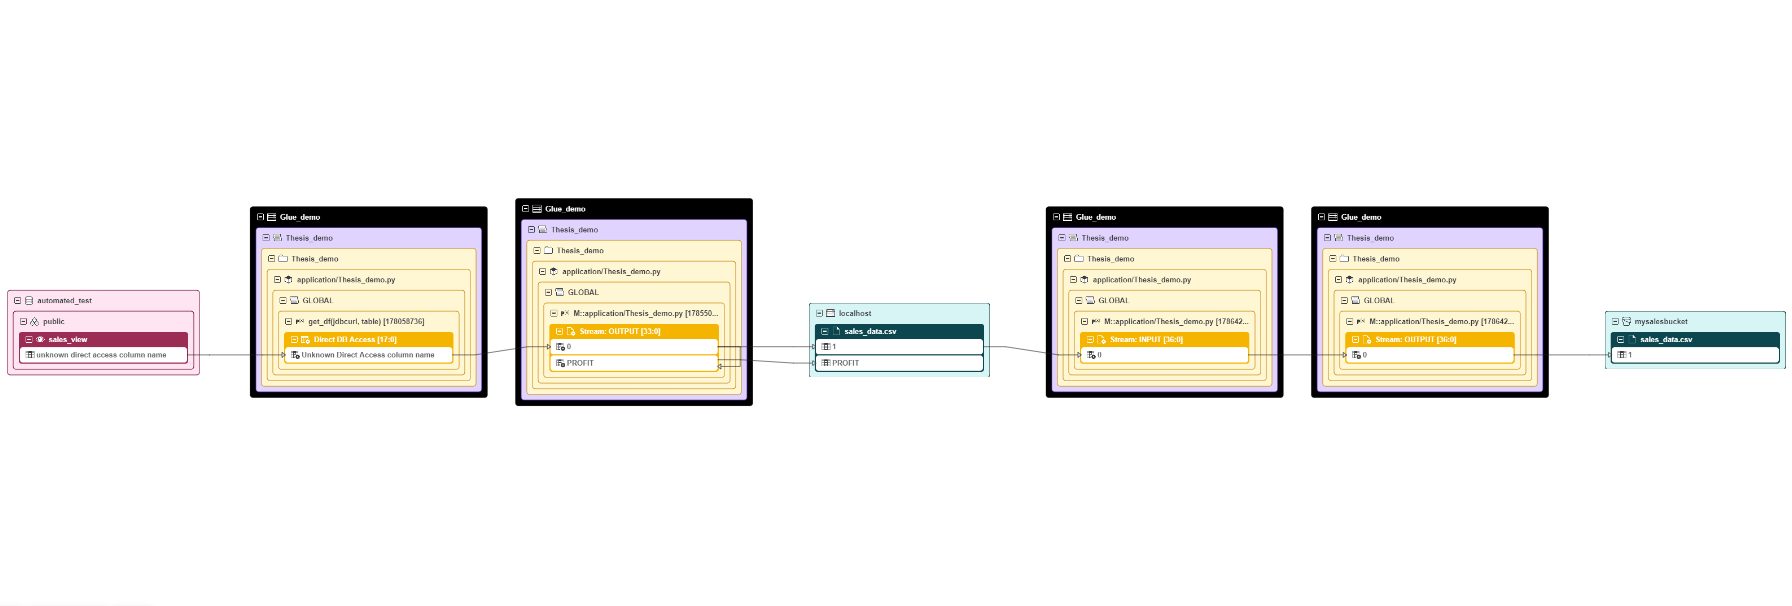
\includegraphics[angle=90,origin=c,height=1.0\textwidth]{img/thesis_demo1.PNG}
\caption{An example of an ETL job created in the graphical tool of AWS Glue}
\label{fig:thesisDemo1}
\end{figure}

\begin{figure}[ht]\centering
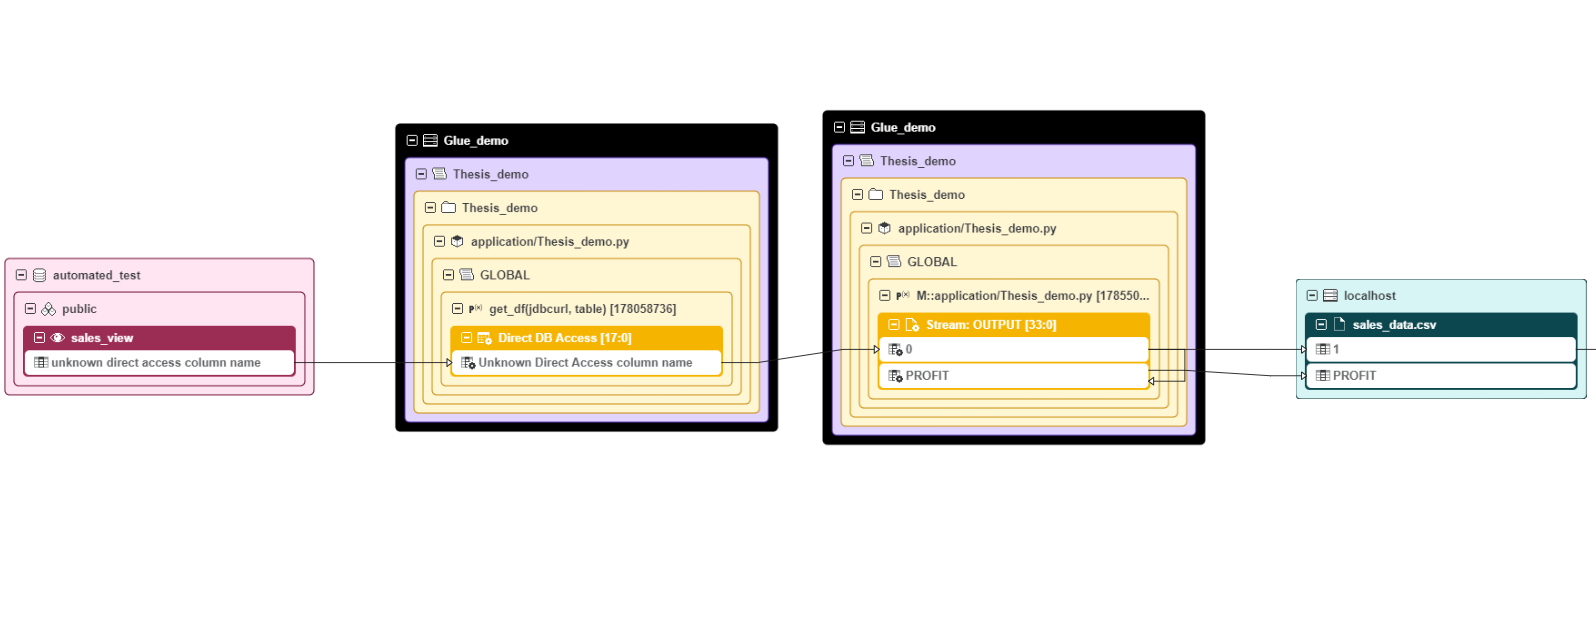
\includegraphics[angle=90,origin=c,height=1.0\textwidth]{img/thesis_demo2.PNG}
\caption{An example of an ETL job created in the graphical tool of AWS Glue}
\label{fig:thesisDemo2}
\end{figure}

\begin{figure}[ht]\centering
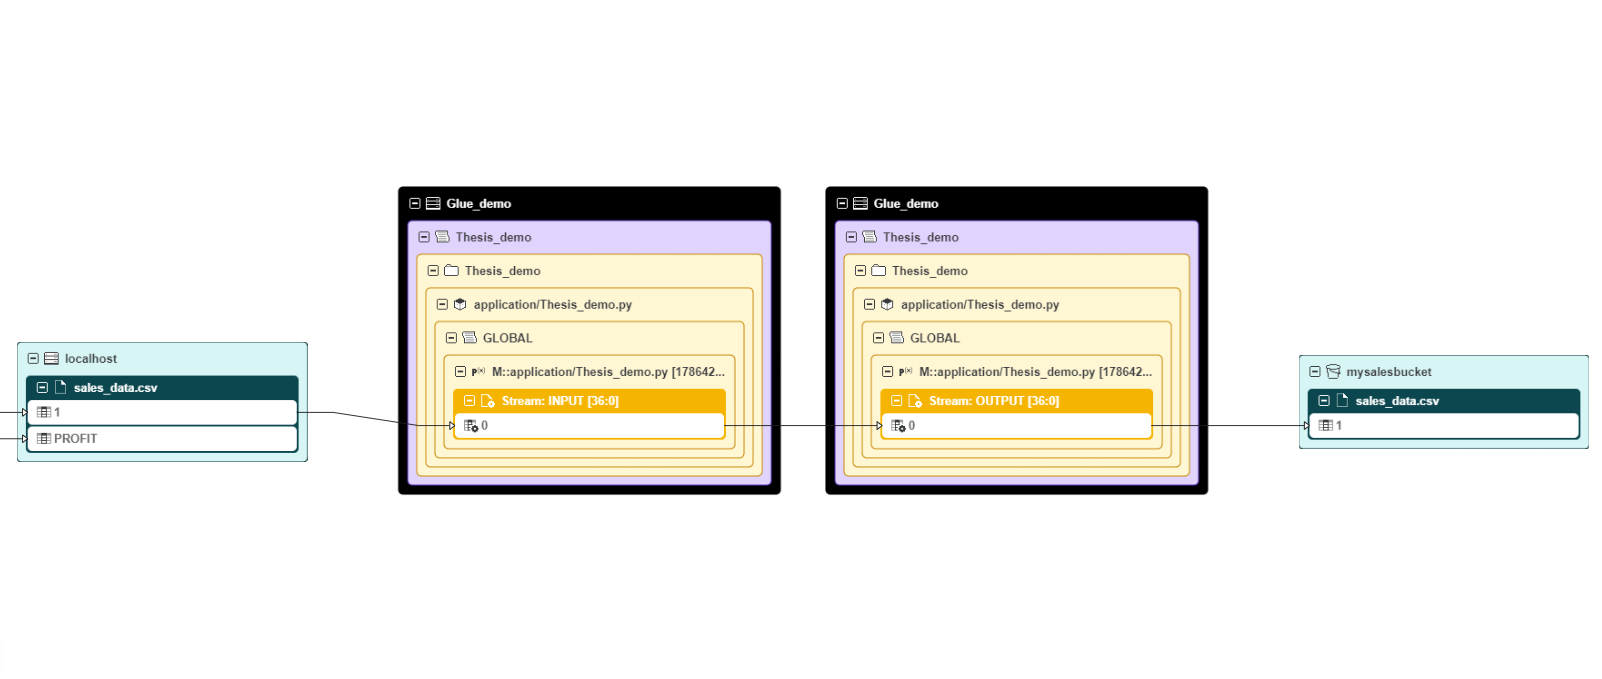
\includegraphics[angle=90,origin=c,height=1.0\textwidth]{img/thesis_demo3.PNG}
\caption{An example of an ETL job created in the graphical tool of AWS Glue}
\label{fig:thesisDemo3}
\end{figure}

\begin{figure}[ht]\centering
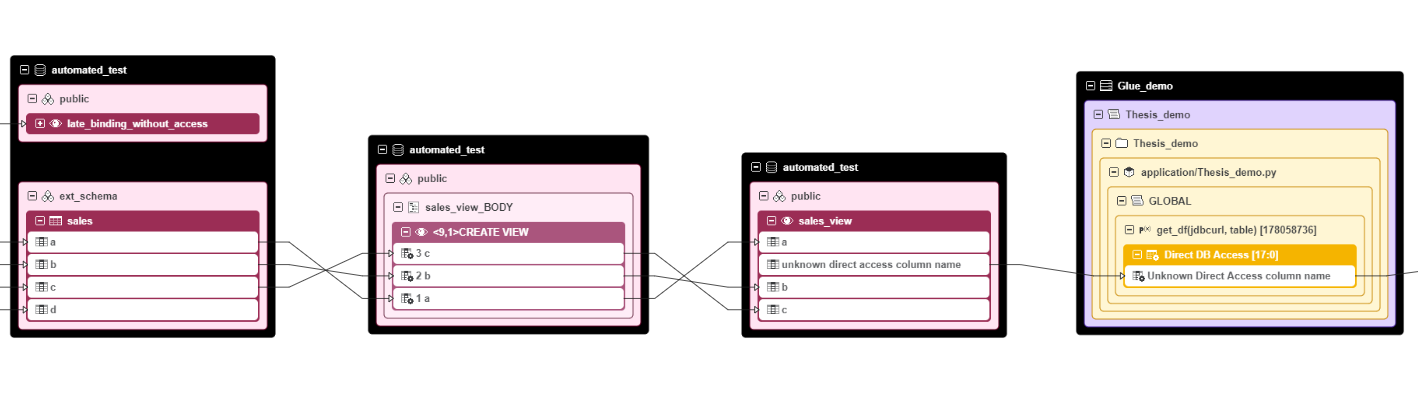
\includegraphics[angle=90,origin=c,height=1.0\textwidth]{img/thesis_demo4.PNG}
\caption{An example of an ETL job created in the graphical tool of AWS Glue}
\label{fig:thesisDemo4}
\end{figure}

\section{Limitations and Future Work}

As demonstrated on the example, Python Embedded Code Service designed and implemented in this work can be integrated with other data technology scanners and is capable of analyzing embedded Python code.

\subsection{Other programming languages}
We have only been able to implement the service for embedded Python code. The analysis of C\# and Java code is not yet supported by any Embedded Code Service. While the implementation was not set as our goal, we have provided a comprehensive guide how these services can be developed should they be required.

\subsection{AWS Glue scanner}
We have developed a prototype of AWS Glue scanner that can analyze data lineage in basic ETL jobs. The range of developed features was sufficient to demonstrate the capabilities of Embedded Code Service, but is not yet sufficient to analyze any inputs provided by customers. 
\par
We have designed several more features that will need to be implemented in the future in order to cover basic capabilities of AWS Glue. Data Catalog analysis is a promising feature to unlock data lineage discovery in AWS Glue. The plugin for \texttt{awsglue} Python library has to be significantly extended to cover more commonly used functions and methods. The further development of the scanner will be a subject to prioritization based on customer preferences.

\subsection{Python scanner improvements}
We have implemented only a few improvements of Python scanner. We needed to redesign several components so the scanner can be integrated with Embedded Code Service and we developed an \texttt{awsglue} library plugin. These changed allowed us to analyze the example script used in this evaluation.
\par
To provide a better value, Python scanner will need to be optimized in the future for the analysis of embedded code. We have observed that embedded Python code is often parameterized, e.g. using job arguments in AWS Glue. Python scanner currently provides poor interface for processing external values and is not optimized to analyze large sets of parameters.

